% Options for packages loaded elsewhere
% Options for packages loaded elsewhere
\PassOptionsToPackage{unicode}{hyperref}
\PassOptionsToPackage{hyphens}{url}
\PassOptionsToPackage{dvipsnames,svgnames,x11names}{xcolor}
%
\documentclass[
  letterpaper,
  DIV=11,
  numbers=noendperiod]{scrreprt}
\usepackage{xcolor}
\usepackage{amsmath,amssymb}
\setcounter{secnumdepth}{5}
\usepackage{iftex}
\ifPDFTeX
  \usepackage[T1]{fontenc}
  \usepackage[utf8]{inputenc}
  \usepackage{textcomp} % provide euro and other symbols
\else % if luatex or xetex
  \usepackage{unicode-math} % this also loads fontspec
  \defaultfontfeatures{Scale=MatchLowercase}
  \defaultfontfeatures[\rmfamily]{Ligatures=TeX,Scale=1}
\fi
\usepackage{lmodern}
\ifPDFTeX\else
  % xetex/luatex font selection
\fi
% Use upquote if available, for straight quotes in verbatim environments
\IfFileExists{upquote.sty}{\usepackage{upquote}}{}
\IfFileExists{microtype.sty}{% use microtype if available
  \usepackage[]{microtype}
  \UseMicrotypeSet[protrusion]{basicmath} % disable protrusion for tt fonts
}{}
\makeatletter
\@ifundefined{KOMAClassName}{% if non-KOMA class
  \IfFileExists{parskip.sty}{%
    \usepackage{parskip}
  }{% else
    \setlength{\parindent}{0pt}
    \setlength{\parskip}{6pt plus 2pt minus 1pt}}
}{% if KOMA class
  \KOMAoptions{parskip=half}}
\makeatother
% Make \paragraph and \subparagraph free-standing
\makeatletter
\ifx\paragraph\undefined\else
  \let\oldparagraph\paragraph
  \renewcommand{\paragraph}{
    \@ifstar
      \xxxParagraphStar
      \xxxParagraphNoStar
  }
  \newcommand{\xxxParagraphStar}[1]{\oldparagraph*{#1}\mbox{}}
  \newcommand{\xxxParagraphNoStar}[1]{\oldparagraph{#1}\mbox{}}
\fi
\ifx\subparagraph\undefined\else
  \let\oldsubparagraph\subparagraph
  \renewcommand{\subparagraph}{
    \@ifstar
      \xxxSubParagraphStar
      \xxxSubParagraphNoStar
  }
  \newcommand{\xxxSubParagraphStar}[1]{\oldsubparagraph*{#1}\mbox{}}
  \newcommand{\xxxSubParagraphNoStar}[1]{\oldsubparagraph{#1}\mbox{}}
\fi
\makeatother


\usepackage{longtable,booktabs,array}
\usepackage{calc} % for calculating minipage widths
% Correct order of tables after \paragraph or \subparagraph
\usepackage{etoolbox}
\makeatletter
\patchcmd\longtable{\par}{\if@noskipsec\mbox{}\fi\par}{}{}
\makeatother
% Allow footnotes in longtable head/foot
\IfFileExists{footnotehyper.sty}{\usepackage{footnotehyper}}{\usepackage{footnote}}
\makesavenoteenv{longtable}
\usepackage{graphicx}
\makeatletter
\newsavebox\pandoc@box
\newcommand*\pandocbounded[1]{% scales image to fit in text height/width
  \sbox\pandoc@box{#1}%
  \Gscale@div\@tempa{\textheight}{\dimexpr\ht\pandoc@box+\dp\pandoc@box\relax}%
  \Gscale@div\@tempb{\linewidth}{\wd\pandoc@box}%
  \ifdim\@tempb\p@<\@tempa\p@\let\@tempa\@tempb\fi% select the smaller of both
  \ifdim\@tempa\p@<\p@\scalebox{\@tempa}{\usebox\pandoc@box}%
  \else\usebox{\pandoc@box}%
  \fi%
}
% Set default figure placement to htbp
\def\fps@figure{htbp}
\makeatother





\setlength{\emergencystretch}{3em} % prevent overfull lines

\providecommand{\tightlist}{%
  \setlength{\itemsep}{0pt}\setlength{\parskip}{0pt}}



 


\KOMAoption{captions}{tableheading}
\makeatletter
\@ifpackageloaded{bookmark}{}{\usepackage{bookmark}}
\makeatother
\makeatletter
\@ifpackageloaded{caption}{}{\usepackage{caption}}
\AtBeginDocument{%
\ifdefined\contentsname
  \renewcommand*\contentsname{Table of contents}
\else
  \newcommand\contentsname{Table of contents}
\fi
\ifdefined\listfigurename
  \renewcommand*\listfigurename{List of Figures}
\else
  \newcommand\listfigurename{List of Figures}
\fi
\ifdefined\listtablename
  \renewcommand*\listtablename{List of Tables}
\else
  \newcommand\listtablename{List of Tables}
\fi
\ifdefined\figurename
  \renewcommand*\figurename{Figure}
\else
  \newcommand\figurename{Figure}
\fi
\ifdefined\tablename
  \renewcommand*\tablename{Table}
\else
  \newcommand\tablename{Table}
\fi
}
\@ifpackageloaded{float}{}{\usepackage{float}}
\floatstyle{ruled}
\@ifundefined{c@chapter}{\newfloat{codelisting}{h}{lop}}{\newfloat{codelisting}{h}{lop}[chapter]}
\floatname{codelisting}{Listing}
\newcommand*\listoflistings{\listof{codelisting}{List of Listings}}
\makeatother
\makeatletter
\makeatother
\makeatletter
\@ifpackageloaded{caption}{}{\usepackage{caption}}
\@ifpackageloaded{subcaption}{}{\usepackage{subcaption}}
\makeatother
\usepackage{bookmark}
\IfFileExists{xurl.sty}{\usepackage{xurl}}{} % add URL line breaks if available
\urlstyle{same}
\hypersetup{
  pdftitle={UTS-5 --- My Personal Reviews},
  pdfauthor={Levina Nathania Bunardi},
  colorlinks=true,
  linkcolor={blue},
  filecolor={Maroon},
  citecolor={Blue},
  urlcolor={Blue},
  pdfcreator={LaTeX via pandoc}}


\title{UTS-5 --- My Personal Reviews}
\usepackage{etoolbox}
\makeatletter
\providecommand{\subtitle}[1]{% add subtitle to \maketitle
  \apptocmd{\@title}{\par {\large #1 \par}}{}{}
}
\makeatother
\subtitle{Portfolio Asesmen II-2100 KIPP}
\author{18224057 Levina Nathania Bunardi}
\date{2025-10-22}
\begin{document}
\maketitle

\renewcommand*\contentsname{Table of contents}
{
\hypersetup{linkcolor=}
\setcounter{tocdepth}{2}
\tableofcontents
}

\bookmarksetup{startatroot}

\chapter*{Hai, apa kabar?}\label{hai-apa-kabar}
\addcontentsline{toc}{chapter}{Hai, apa kabar?}

\markboth{Hai, apa kabar?}{Hai, apa kabar?}

\begin{figure}[H]

{\centering 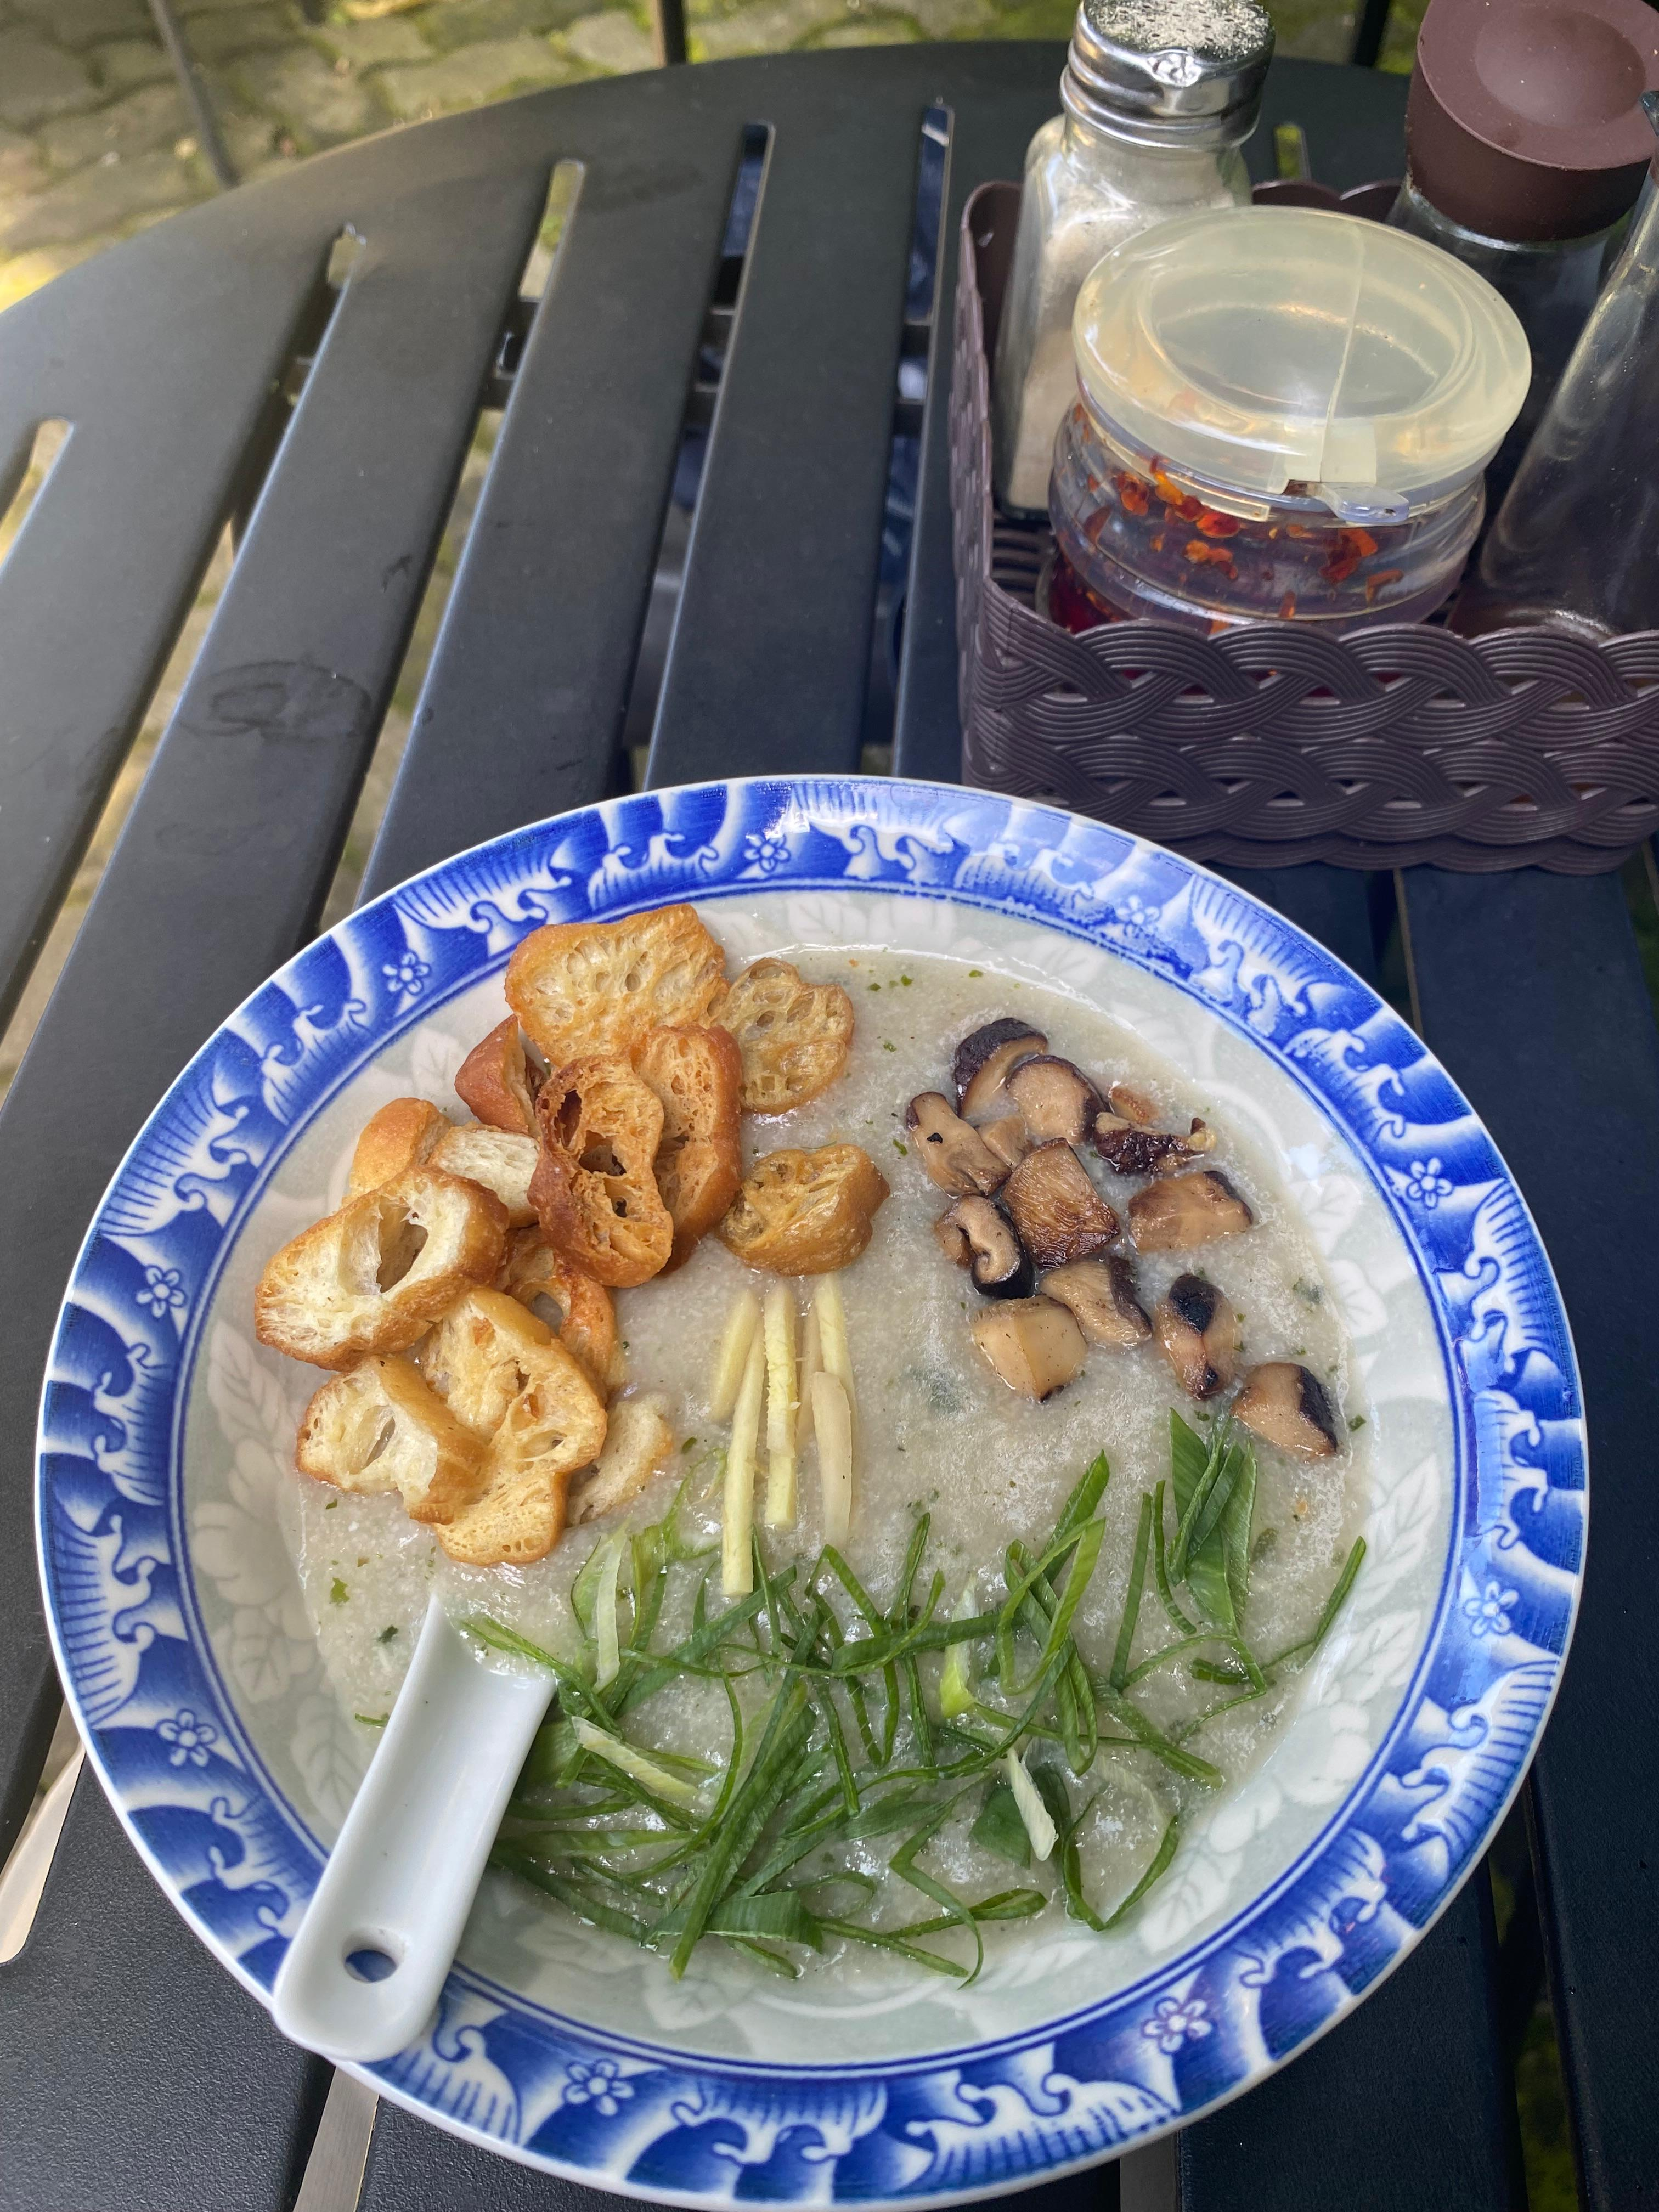
\includegraphics[width=1\linewidth,height=\textheight,keepaspectratio]{images/bubur.png}

}

\caption{About Me}

\end{figure}%

Halo! Nama saya Levina Nathania Bunardi, asal Jakarta, dan saya seorang
mahasiswa STI STEI-K yang saat ini sedang menempuh semester 3. Saya
memiliki ketertarikan besar pada dunia teknologi dan pengembangan diri,
khususnya dalam memahami bagaimana teknologi bisa membantu kehidupan
sehari-hari jadi lebih efisien dan bermanfaat. Selama perkuliahan, saya
berusaha untuk terus belajar, beradaptasi, dan mengasah kemampuan
berpikir kritis maupun kolaboratif.

Di luar kegiatan akademik, saya suka mencoba hal-hal baru yang bisa
menambah pengalaman dan wawasan, baik melalui kegiatan kampus, UKM (Unit
Kegiatan Mahasiswa), maupun diskusi dengan teman-teman. Saya percaya
bahwa setiap proses belajar, sekecil apa pun, akan memberikan nilai
tambah yang berarti untuk perjalanan saya ke depan.

\bookmarksetup{startatroot}

\chapter{UTS-1 All About Me}\label{uts-1-all-about-me}

\begin{figure}[H]

{\centering 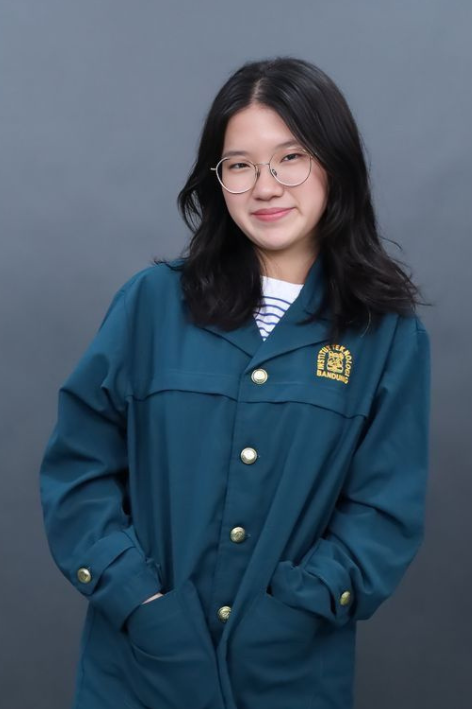
\includegraphics[width=3\linewidth,height=\textheight,keepaspectratio]{All_About_me/../images/Foto_18224057_Levina Nathania Bunardi.png}

}

\caption{Pieces of My Journey}

\end{figure}%

Halo! Nama saya Levina Nathania Bunardi, asal Jakarta, dan saya seorang
mahasiswa Sistem dan Teknologi Informasi ITB yang saat ini sedang
menempuh semester 3. Saya memiliki ketertarikan besar terhadap dunia
teknologi dan pengembangan diri, terutama dalam memahami bagaimana
teknologi dapat membantu kehidupan sehari-hari menjadi lebih efisien,
bermakna, dan manusiawi. Selama perkuliahan, saya berusaha untuk terus
belajar dan beradaptasi, baik di ruang kelas maupun di luar, sambil
mengasah kemampuan berpikir kritis, kolaboratif, dan empatik agar dapat
menjadi pribadi yang tidak hanya unggul secara akademik, tetapi juga
peka terhadap orang lain.

Di luar kegiatan akademik, saya senang mencoba hal-hal baru yang bisa
menambah pengalaman dan memperluas wawasan. Kegiatan tersebut bisa
berupa mengikuti acara kampus, bergabung dalam Unit Kegiatan Mahasiswa,
atau sekadar berdiskusi santai bersama teman-teman di kantin ITB yang
entah bagaimana sering berujung pada obrolan reflektif menjelang malam.
Saya percaya setiap interaksi, sekecil apa pun, memiliki daya tarik
tersendiri. Kadang bukan karena topiknya yang menarik, tetapi karena
orang yang terlibat di dalamnya punya karakter dan keaslian yang
memikat. Dari situ saya belajar bahwa daya tarik interpersonal tidak
hanya bergantung pada penampilan atau gaya bicara, melainkan juga pada
ketulusan, humor yang tepat, dan kemampuan membuat orang lain merasa
nyaman.

Saya juga memiliki pengalaman tragis tapi lucu saat masih di bangku SMA.
Waktu itu, saya patah kaki karena ujian praktikum lompat tali. Ya,
benar, lompat tali. Ironisnya, saya begitu bersemangat saat itu, tapi
justru berakhir dengan kaki digips selama tiga bulan penuh. Sekilas
terdengar konyol, tetapi pengalaman itu justru memberikan banyak
pelajaran berharga. Selama masa pemulihan, saya benar-benar merasakan
betapa besar arti dukungan keluarga dan teman-teman. Dari peristiwa itu
saya belajar bahwa daya tarik seseorang tidak selalu muncul dari
kesempurnaan, melainkan juga dari kerentanan dan kejujuran dalam
menghadapi kesulitan. Perhatian kecil, candaan ringan, atau sekadar
kehadiran seseorang bisa menjadi sumber kekuatan yang luar biasa.

Bagi saya, perjalanan ini bukan hanya tentang menempuh pendidikan di
bidang teknologi, tetapi juga tentang memahami manusia di balik
teknologi itu sendiri. Saya ingin tahu bagaimana kita dapat menciptakan
solusi yang lebih empatik, lebih dekat dengan kebutuhan nyata, dan tetap
menghadirkan kehangatan di tengah dunia yang semakin digital. Dan
mungkin, jika suatu hari nanti saya bisa melompat tali lagi tanpa
insiden, itu akan menjadi simbol kemajuan saya. Bukan hanya dalam
keseimbangan tubuh, tetapi juga dalam keseimbangan hidup.

\bookmarksetup{startatroot}

\chapter{UTS-2 My Songs for You}\label{uts-2-my-songs-for-you}

Verse 1 We came with wounds unhealed, carrying nights that never slept.
Through quiet eyes and trembling hands, we found the strength to gently
weep.

The world feels cold sometimes, and mercy wears a fragile face. Yet even
through our brokenness, we still can offer grace.

Pre-Chorus Maybe love was never clean, never bound to what's serene.
Maybe kindness softly shines, in hands that shake but still entwine.

Chorus Still, we can be kind, even when the light feels small. Still, we
can be true, though we may stumble and fall. For love is not perfection
found, but peace in hearts that stay around. We're not always whole, but
we can still be kind.

Verse 2 We walk through echoes of regret, with voices whispering our
name. And still we offer gentle words, like light that flickers through
the rain.

Perhaps the pure are just the brave, who choose to love through pain.
Who see the world in shades of grey, yet still believe in grace again.

Pre-Chorus If all that's left are tears to give, let them fall, let them
forgive. For cleansing never needs to shine, it only needs to feel
divine.

Chorus Still, we can be kind, even when our hearts feel worn. Still, we
can be true, though our edges are torn. For love was never meant to
bind, but to free the tender mind. We're not always whole, but we can
still be kind.

Bridge Let the tears fall freely down, they're proof we're still alive.
Let the silence hold our sound, like dawn that dares to rise. In every
crack, the light will grow, and in our flaws, compassion shows. Still,
we can be kind.

Final Chorus Still, we can be kind, even when the world forgets. Still,
we can be true, when forgiveness feels like debt. For love remains,
though torn by time, a gentle echo, pure and fine. We're not always
whole, but we can still be kind.

Outro Still, we can be kind. Still, we can be kind.

\bookmarksetup{startatroot}

\chapter{UTS-3 My Stories for You}\label{uts-3-my-stories-for-you}

Sesuatu di Malang

Setelah menghabiskan pagi dan siang hari di dalam satu ruangan yang
terasa begitu padat dengan berbagai kegiatan, akhirnya kami bertiga bisa
keluar untuk menghirup udara segar Malang. Kota ini selalu punya cara
sendiri untuk menenangkan, entah lewat semilir anginnya atau aroma
makanan yang menggoda di setiap sudut jalan. Kami memutuskan untuk pergi
makan siang bersama, mencoba kuliner khas Malang yang katanya wajib
dicoba oleh siapa pun yang datang ke kota ini, tentu saja bakso malang.
Suasana makan siang terasa ringan dan menyenangkan, kami saling
bercerita, tertawa kecil, dan menikmati waktu tanpa terburu-buru.
Setelahnya, kami mampir ke sebuah kafe yang tenang untuk beristirahat
sejenak. Di sana, kami tidak melakukan apa-apa selain bersandar, menatap
langit yang mulai meredup, dan membiarkan tubuh beristirahat dari
rutinitas yang padat sejak pagi. Menjelang sore, sekitar pukul setengah
lima, kami berpisah sejenak untuk menuju rumah ibadah masing-masing. Ada
rasa damai yang menenangkan ketika selesai berdoa sebelum kembali
melanjutkan hari. Setelah itu, kami berkumpul lagi di Universitas
Brawijaya, tempat di mana acara malam itu akan diadakan. Di antara kami
bertiga, saya datang paling lambat, dua teman saya sudah menunggu sambil
mengobrol ringan di parkiran. Kami sempat bercanda kecil sebelum
akhirnya dijemput oleh seseorang dari panitia acara. Ia menyambut kami
dengan ramah, lalu membawa kami menuju lokasi yang ternyata tidak
terlalu jauh. Sesampainya di tempat acara, suasananya langsung terasa
berbeda. Ada campuran antara rasa penasaran, antusias, dan sedikit kagum
melihat betapa rapi dan hangatnya penyambutan malam itu. Sebelum acara
dimulai, kami dihidangkan makan malam yang begitu nikmat, sepiring rawon
dengan kuah hitam pekat disajikan bersama nasi hangat yang aromanya saja
sudah cukup membuat perut bergejolak. Rasa lelah seharian langsung
terbayar. Setelah makan malam, kami diarahkan masuk ke ruangan utama.
Pencahayaan lembut, dekorasi elegan, dan alunan musik pelan membuat
suasananya terasa akrab dan menyenangkan. Semua orang tampak menikmati
momen itu, tersenyum, bercakap, dan saling menyapa satu sama lain. Acara
dimulai dengan sesi talkshow dari salah satu tokoh penting Telkomsel. Ia
berbicara tentang perjalanan, semangat, dan nilai yang sering kali
terlupakan dalam proses menuju tujuan. Ucapannya sederhana tapi dalam.
Ia menekankan bahwa yang membuat seseorang berharga bukanlah hasil
akhirnya, tapi usaha yang dijalani, keberanian untuk gagal, dan
kesediaan untuk terus belajar. Saya mendengarkannya dengan saksama, dan
entah kenapa, kalimat-kalimat itu terasa menempel di kepala saya hingga
sekarang. Ada semacam dorongan untuk terus maju, untuk terus ingin
berkembang dan memberi arti. Setelah sesi utama selesai, suasana menjadi
jauh lebih cair. Musik pelan mulai terdengar, orang-orang mulai bergerak
dari kursinya, dan tawa mulai memenuhi ruangan. Bagi saya, inilah bagian
terbaik dari malam itu, momen di mana saya bisa berinteraksi dengan
banyak orang baru. Saya bertemu dengan mahasiswa dari berbagai daerah,
panitia yang energik dan penuh semangat, serta beberapa tamu yang punya
cerita menarik tentang perjalanan hidup mereka. Kami saling bertukar
pandangan, berbagi pengalaman, bahkan sesekali tertawa bersama karena
hal-hal kecil yang lucu. Ada kehangatan yang sulit dijelaskan, semacam
rasa saling menghargai meski baru saja bertemu. Saya pulang malam itu
dengan hati yang penuh. Udara Malang yang dingin terasa lebih hangat
dari biasanya. Saya berjalan menuju kendaraan sambil tersenyum kecil,
memutar kembali setiap percakapan dan momen yang baru saja terjadi. Bagi
sebagian orang, mungkin itu hanya sebuah acara malam biasa. Tapi bagi
saya, itu adalah pengalaman berharga, malam yang sederhana namun penuh
makna. Saya belajar bahwa terkadang, kebahagiaan tidak datang dari
hal-hal besar, tapi dari pertemuan yang tulus, tawa yang ringan, dan
kesempatan untuk merasa terhubung dengan orang lain. Malam itu bukan
sekadar penutup hari yang panjang, tapi pengingat bahwa setiap pertemuan
punya cara sendiri untuk mengajarkan sesuatu.

\bookmarksetup{startatroot}

\chapter{UTS-4 My SHAPE (Spiritual Gifts, Heart, Abilities, Personality,
Experiences)}\label{uts-4-my-shape-spiritual-gifts-heart-abilities-personality-experiences}

\bookmarksetup{startatroot}

\chapter{UTS-4 --- My SHAPE}\label{uts-4-my-shape}

\emph{(Spiritual Gifts, Heart, Abilities, Personality, Experiences)}

Halo! Nama saya \textbf{Levina Nathania Bunardi}, asal Jakarta, dan saya
mahasiswa \textbf{Program Studi Sistem dan Teknologi Informasi (STI)
ITB} semester 3.\\
Saya memiliki ketertarikan besar pada dunia \textbf{teknologi dan
pengembangan diri}, terutama bagaimana teknologi dapat membantu
kehidupan sehari-hari menjadi lebih efisien dan bermakna.\\
Sebagai mahasiswa, saya belajar untuk menyeimbangkan antara fokus
akademik dan eksplorasi hal-hal baru di luar perkuliahan.\\
Saya percaya bahwa proses belajar tidak hanya terjadi di ruang kelas,
tetapi juga melalui pengalaman, interaksi, dan waktu refleksi diri.

Di luar kegiatan akademik, saya menikmati aktivitas yang berhubungan
dengan \textbf{benang}, seperti \emph{crochet}, \emph{knitting}, dan
\emph{tatting}.\\
Kegiatan ini membantu saya melatih kesabaran, fokus, serta ketelitian
--- kualitas yang juga sangat berguna dalam dunia teknologi.\\
Bagi saya, setiap simpul benang memiliki filosofi: hasil yang indah
tidak datang dari kecepatan, tetapi dari konsistensi dan ketekunan dalam
proses.

\begin{center}\rule{0.5\linewidth}{0.5pt}\end{center}

\section{4.1 Sumber --- VIA Character Strengths
Profile}\label{sumber-via-character-strengths-profile}

Berdasarkan hasil \textbf{VIA Character Strengths Profile (22 Oktober
2025)}, sepuluh kekuatan utama saya adalah:

\begin{enumerate}
\def\labelenumi{\arabic{enumi}.}
\tightlist
\item
  Forgiveness (Memaafkan)\\
\item
  Kindness (Kebaikan Hati)\\
\item
  Hope (Harapan)\\
\item
  Humility (Kerendahan Hati)\\
\item
  Gratitude (Rasa Syukur)\\
\item
  Fairness (Keadilan)\\
\item
  Judgment (Kebijaksanaan dalam Menilai)\\
\item
  Honesty (Kejujuran)\\
\item
  Love (Kasih)\\
\item
  Love of Learning (Suka Belajar)
\end{enumerate}

Kombinasi kekuatan ini menunjukkan bahwa saya cenderung reflektif,
empatik, dan berorientasi pada hubungan manusia.\\
Dalam konteks akademik, hal ini membantu saya membangun kerja tim yang
harmonis, terbuka terhadap umpan balik, dan fokus pada kolaborasi yang
produktif.

\begin{center}\rule{0.5\linewidth}{0.5pt}\end{center}

\section{4.2 0) Ringkasan 1 Halaman}\label{ringkasan-1-halaman}

\textbf{Peran Inti:}\\
Mahasiswa reflektif yang berorientasi pada pengembangan diri dan
keseimbangan antara logika serta empati.

\textbf{Misi:}\\
Mengintegrasikan kemampuan analitis, empati, dan kreativitas untuk
menciptakan pembelajaran serta karya yang berdampak positif di bidang
teknologi dan kehidupan sosial.

\textbf{Kekuatan Utama:}\\
Rasa syukur, empati, keadilan, dan semangat belajar.

\textbf{Dampak yang Dituju:}\\
Menjadi pribadi yang berpikir kritis, bertanggung jawab, dan mampu
beradaptasi sambil tetap menjaga nilai-nilai kemanusiaan dalam setiap
proses belajar.

\begin{center}\rule{0.5\linewidth}{0.5pt}\end{center}

\section{4.3 1) S --- Spiritual Gifts (Karunia
Rohani)}\label{s-spiritual-gifts-karunia-rohani}

Saya merasa karunia utama saya ada pada kemampuan \textbf{mendengarkan,
memahami, dan memberi empati} kepada orang lain.\\
Dalam kelompok, saya sering menjadi penyeimbang --- memastikan semua
anggota punya ruang bicara dan merasa dihargai.\\
Saya percaya bahwa mendengarkan adalah bentuk pelayanan yang sederhana
tapi bermakna, karena dari situ kita bisa benar-benar memahami kebutuhan
orang lain.

Dalam konteks rohani, saya ingin terus belajar untuk menjadi pribadi
yang rendah hati, tidak cepat menilai, dan mau belajar dari sudut
pandang yang berbeda.\\
Saya percaya bahwa kebijaksanaan tidak datang dari banyaknya bicara,
tapi dari kemampuan memahami dengan hati.

\begin{center}\rule{0.5\linewidth}{0.5pt}\end{center}

\section{4.4 2) H --- Heart (Minat \&
Passion)}\label{h-heart-minat-passion}

Saya memiliki minat besar pada \textbf{teknologi dan desain sistem
informasi} --- bagaimana teknologi dapat diolah menjadi solusi yang
manusiawi.\\
Saya tertarik pada bidang yang melibatkan kombinasi antara logika,
kreativitas, dan empati.\\
Selain itu, saya menemukan kepuasan dalam kegiatan \textbf{kerajinan
benang} seperti crochet dan knitting.\\
Bagi saya, aktivitas itu bukan sekadar hobi, tapi sarana refleksi diri
dan latihan kesabaran.

Kedua dunia ini --- teknologi dan kerajinan --- memberi keseimbangan
bagi saya: teknologi mengasah cara berpikir terstruktur, sementara
kerajinan melatih intuisi dan kesadaran detail.\\
Saya merasa paling hidup ketika bisa menggabungkan keduanya --- berpikir
kritis sambil tetap kreatif dan tenang.

\begin{center}\rule{0.5\linewidth}{0.5pt}\end{center}

\section{4.5 3) A --- Abilities
(Kemampuan)}\label{a-abilities-kemampuan}

Selama tiga semester kuliah di STI ITB, saya mulai mengenali beberapa
kemampuan yang berkembang:

\begin{itemize}
\tightlist
\item
  \textbf{Kemampuan analitis dan berpikir sistematis}, terutama dalam
  memahami struktur masalah.\\
\item
  \textbf{Kemampuan reflektif}, yaitu meninjau ulang keputusan dan
  belajar dari pengalaman.\\
\item
  \textbf{Kemampuan komunikasi tertulis dan lisan}, yang terasah lewat
  diskusi dan tugas kelompok.\\
\item
  \textbf{Kemampuan manajemen waktu dan tanggung jawab akademik}, agar
  tetap seimbang antara tugas, kegiatan kampus, dan waktu istirahat.
\end{itemize}

Saya juga senang belajar hal baru secara mandiri --- seperti mencoba
bahasa pemrograman baru atau memahami sistem dengan pendekatan logika.\\
Saya masih terus mengembangkan keberanian untuk tampil di depan publik
dan menyampaikan ide dengan percaya diri.

\begin{center}\rule{0.5\linewidth}{0.5pt}\end{center}

\section{4.6 4) P --- Personality
(Kepribadian)}\label{p-personality-kepribadian}

Saya termasuk tipe \textbf{reflektif, tenang, dan rasional}, tetapi juga
mudah berempati terhadap orang lain.\\
Saya lebih suka memahami konteks secara utuh sebelum mengambil
keputusan.\\
Dalam tim, saya berusaha menjaga suasana tetap stabil dan saling
menghargai.

Kepribadian ini membantu saya untuk tidak reaktif, tetapi berpikir
matang sebelum bertindak.\\
Meski cenderung introvert, saya menikmati kerja kelompok yang
komunikatif.\\
Saya belajar bahwa menjadi tenang bukan berarti diam, tetapi fokus
mencari solusi yang realistis dan damai.

\begin{center}\rule{0.5\linewidth}{0.5pt}\end{center}

\section{4.7 5) E --- Experiences
(Pengalaman)}\label{e-experiences-pengalaman}

Sejauh ini, pengalaman kuliah dan organisasi membantu saya banyak
belajar tentang diri sendiri.\\
Saya pernah terlibat dalam proyek kelompok di mana saya berperan
mengatur pembagian tugas dan memastikan semua anggota memahami
perannya.\\
Dari situ saya belajar pentingnya komunikasi terbuka dan kejelasan
struktur kerja.

Selain itu, saya juga belajar mengatur keseimbangan antara tugas
akademik dan hobi pribadi seperti crochet.\\
Kegiatan ini membantu saya tetap tenang di tengah kesibukan akademik,
sekaligus memberi ruang bagi refleksi diri.\\
Saya merasa setiap pengalaman --- baik akademik maupun personal ---
adalah bagian penting dari proses menemukan jati diri saya.

\begin{center}\rule{0.5\linewidth}{0.5pt}\end{center}

\section{4.8 6) Piagam Diri
(Self-Charter)}\label{piagam-diri-self-charter}

\textbf{Misi Hidup:}\\
Belajar dengan tekun, bertumbuh dengan rendah hati, dan membagikan
kebaikan melalui pengetahuan dan karya.

\textbf{Nilai Inti:}\\
Kejujuran • Empati • Ketekunan • Rasa Syukur • Keadilan • Keseimbangan.

\textbf{Peran Inti:}\\
Mahasiswa yang belajar bukan hanya untuk nilai, tetapi untuk memahami,
berkontribusi, dan menginspirasi orang lain.

\textbf{Kompas Keputusan:}\\
1. Apakah keputusan ini membantu saya tumbuh secara akademik dan
moral?\\
2. Apakah tindakan ini selaras dengan nilai empati dan kejujuran?\\
3. Apakah hasilnya memberi manfaat bagi diri sendiri maupun orang lain?

\textbf{Janji Pribadi:}\\
Untuk menjaga konsistensi belajar, berpikir dengan hati dan logika,
serta menghargai setiap proses --- sekecil apa pun hasilnya.

\begin{center}\rule{0.5\linewidth}{0.5pt}\end{center}

\section{4.9 7) Narasi 90 Detik (Elevator
Pitch)}\label{narasi-90-detik-elevator-pitch}

``Halo, saya \textbf{Levina}, mahasiswa semester 3 Program Studi Sistem
dan Teknologi Informasi ITB.\\
Saya sedang dalam proses menemukan arah dan potensi diri, sambil
mendalami bagaimana teknologi bisa memberi dampak positif bagi
kehidupan.

Saya percaya bahwa belajar bukan hanya tentang teori, tapi juga tentang
mengenali nilai-nilai yang membentuk diri.\\
Saya senang menganalisis, menulis, dan berkolaborasi, tapi juga
menyeimbangkannya dengan aktivitas seperti crochet dan knitting ---
karena dari situ saya belajar ketekunan dan fokus.

Ke depan, saya ingin menjadi pribadi yang tidak hanya kompeten secara
teknis, tapi juga peka terhadap manusia dan lingkungan sekitar.\\
Bagi saya, teknologi yang terbaik adalah yang membawa manfaat nyata dan
membuat hidup lebih bermakna.''

\begin{center}\rule{0.5\linewidth}{0.5pt}\end{center}

\section{4.10 8) Rencana Aksi 90 Hari
(SMART)}\label{rencana-aksi-90-hari-smart}

\begin{enumerate}
\def\labelenumi{\arabic{enumi}.}
\item
  \textbf{Menyusun refleksi mingguan tentang proses belajar di STI
  ITB.}\\
  \emph{Outcome:} Minimal 4 tulisan reflektif yang menunjukkan perubahan
  pola pikir.\\
  \emph{Due:} 45 hari.
\item
  \textbf{Mengikuti satu kegiatan atau kompetisi akademik bidang
  teknologi.}\\
  \emph{Outcome:} Laporan pengalaman dan pembelajaran yang diperoleh.\\
  \emph{Due:} 75 hari.
\item
  \textbf{Membuat karya crochet bertema ``Growth'' dan menulis refleksi
  maknanya.}\\
  \emph{Outcome:} Karya fisik + tulisan 300 kata tentang ketekunan dan
  proses.\\
  \emph{Due:} 90 hari.
\end{enumerate}

\begin{center}\rule{0.5\linewidth}{0.5pt}\end{center}

\section{4.11 9) Self-Assessment Rubrik
UTS-4}\label{self-assessment-rubrik-uts-4}

\begin{longtable}[]{@{}
  >{\raggedright\arraybackslash}p{(\linewidth - 6\tabcolsep) * \real{0.2029}}
  >{\raggedright\arraybackslash}p{(\linewidth - 6\tabcolsep) * \real{0.5145}}
  >{\centering\arraybackslash}p{(\linewidth - 6\tabcolsep) * \real{0.1232}}
  >{\raggedright\arraybackslash}p{(\linewidth - 6\tabcolsep) * \real{0.1594}}@{}}
\toprule\noalign{}
\begin{minipage}[b]{\linewidth}\raggedright
\textbf{Kriteria}
\end{minipage} & \begin{minipage}[b]{\linewidth}\raggedright
\textbf{Deskripsi}
\end{minipage} & \begin{minipage}[b]{\linewidth}\centering
\textbf{Skor (1--5)}
\end{minipage} & \begin{minipage}[b]{\linewidth}\raggedright
\textbf{Bukti / Catatan}
\end{minipage} \\
\midrule\noalign{}
\endhead
\bottomrule\noalign{}
\endlastfoot
Kelengkapan SHAPE & Semua aspek S-H-A-P-E telah terisi dengan cukup
lengkap dan relevan. & \textbf{4} & Ada keseimbangan antara akademik dan
refleksi personal. \\
Koherensi Piagam Diri & Misi dan nilai pribadi tergambar jelas dan
konsisten. & \textbf{4} & Nilai inti dan kompas keputusan logis \&
realistis. \\
Narasi 90 Detik & Narasi personal mengalir, jujur, dan merefleksikan
identitas diri. & \textbf{5} & Relevan dengan konteks mahasiswa STI
ITB. \\
Evidence \& Aksi 90 Hari & Rencana SMART konkret, tapi masih perlu
metrik hasil lebih terukur. & \textbf{3} & Tujuan sudah jelas, perlu
indikator capaian lebih spesifik. \\
\end{longtable}

\textbf{Total (maks 20): 16/20}\\
\textbf{Tingkat:} \textbf{B (70--84\%)}

\begin{center}\rule{0.5\linewidth}{0.5pt}\end{center}

\section{4.12 Versi Ultra-Ringkas (≤ 140
kata)}\label{versi-ultra-ringkas-140-kata}

``Saya \textbf{Levina}, mahasiswa Sistem dan Teknologi Informasi ITB
semester 3 yang sedang mengeksplorasi arah dan potensi diri.\\
Saya punya ketertarikan pada teknologi, analisis sistem, dan kegiatan
kreatif seperti crochet dan knitting.\\
Bagi saya, belajar adalah proses yang berkelanjutan --- bukan hanya
untuk nilai, tapi untuk memahami diri dan memberi makna bagi orang
lain.\\
Kekuatan saya terletak pada empati, ketekunan, dan semangat belajar yang
tinggi.\\
Ke depan, saya ingin terus bertumbuh menjadi pribadi yang seimbang:
cakap dalam berpikir logis, tapi tetap hangat dan peka terhadap
sesama.''

\bookmarksetup{startatroot}

\chapter{UTS-5 My Personal Reviews}\label{uts-5-my-personal-reviews}

\bookmarksetup{startatroot}

\chapter{My Personal Reviews}\label{my-personal-reviews}

\textbf{Nama Penulis:} Levina Nathania Bunardi\\
\textbf{Penilai:} Evaluasi Mandiri

\begin{center}\rule{0.5\linewidth}{0.5pt}\end{center}

\section{Gambaran Umum}\label{gambaran-umum}

Portfolio UTS ini disusun dengan baik dan mencerminkan refleksi diri
yang matang.\\
Seluruh komponen yang diminta \textbf{All About Me}, \textbf{My Songs
for You}, \textbf{My Stories for You}, \textbf{My SHAPE}, dan \textbf{My
Personal Reviews} tersaji dengan runtut dan saling melengkapi.

Website memiliki navigasi yang jelas serta gaya bahasa yang lembut,
reflektif, dan konsisten.\\
Secara keseluruhan, karya ini menunjukkan proses pertumbuhan pribadi
yang alami dari seorang mahasiswa semester tiga yang sedang mengenali
potensi serta arah pengembangan dirinya.

\begin{center}\rule{0.5\linewidth}{0.5pt}\end{center}

\section{Penilaian per Bagian (Berdasarkan
Rubrik)}\label{penilaian-per-bagian-berdasarkan-rubrik}

\subsection{UTS 1 --- All About Me}\label{uts-1-all-about-me-1}

\begin{itemize}
\tightlist
\item
  \textbf{Orisinalitas:} 4 -- Tulisan memperlihatkan kejujuran diri dan
  terasa natural tanpa dibuat-buat.\\
\item
  \textbf{Keterlibatan:} 4 -- Gaya narasi ringan dan mudah diikuti,
  meskipun bisa diperkuat dengan contoh nyata dari kehidupan kampus.\\
\item
  \textbf{Humor:} 3 -- Nada tulisan reflektif, namun tetap hangat dan
  mudah didekati.\\
\item
  \textbf{Wawasan:} 5 -- Memberikan pandangan yang jelas tentang
  perkembangan diri melalui proses belajar dan adaptasi.
\end{itemize}

\textbf{Total:} 16/20 (\textbf{80\%})

\textbf{Catatan Perbaikan:}\\
Dapat menambahkan pengalaman spesifik dari kegiatan kampus untuk
memperkuat keterhubungan antara refleksi dan realita.

\begin{center}\rule{0.5\linewidth}{0.5pt}\end{center}

\subsection{UTS 2 --- My Songs for You}\label{uts-2-my-songs-for-you-1}

\begin{itemize}
\tightlist
\item
  \textbf{Orisinalitas:} 5 -- Puisi yang terinspirasi dari lagu
  \emph{Membasuh} menampilkan interpretasi pribadi yang kuat dan penuh
  makna.\\
\item
  \textbf{Keterlibatan:} 5 -- Bahasa puitisnya halus dan mengalir,
  menciptakan kesan emosional yang mendalam.\\
\item
  \textbf{Humor:} N/A -- Karya bersifat reflektif dan emosional.\\
\item
  \textbf{Inspirasi:} 5 -- Menyampaikan pesan tulus tentang kasih, luka,
  dan keteguhan hati dengan cara yang sederhana namun menyentuh.
\end{itemize}

\textbf{Total:} 18/20 (\textbf{90\%})

\textbf{Catatan Perbaikan:}\\
Menambahkan pengantar singkat mengenai alasan pemilihan lagu dapat
memperkuat konteks dan relevansi puisi.

\begin{center}\rule{0.5\linewidth}{0.5pt}\end{center}

\subsection{UTS 3 --- My Stories for
You}\label{uts-3-my-stories-for-you-1}

\begin{itemize}
\tightlist
\item
  \textbf{Orisinalitas:} 5 -- Cerita pengalaman di Malang terasa
  autentik dan disampaikan dengan detail yang hidup.\\
\item
  \textbf{Keterlibatan:} 5 -- Deskripsi suasana, emosi, dan interaksi
  ditulis dengan apik, membuat pembaca ikut larut dalam cerita.\\
\item
  \textbf{Pengembangan Narasi:} 5 -- Struktur narasi lengkap, dengan
  alur yang runtut dari awal hingga refleksi penutup.\\
\item
  \textbf{Inspirasi:} 4 -- Cerita menyampaikan pesan hangat tentang
  kebersamaan, rasa syukur, dan makna sederhana dalam pertemuan.
\end{itemize}

\textbf{Total:} 19/20 (\textbf{95\%})

\textbf{Catatan Perbaikan:}\\
Dapat menambahkan refleksi pribadi tambahan tentang bagaimana pengalaman
tersebut memengaruhi pandangan atau semangat belajar.

\begin{center}\rule{0.5\linewidth}{0.5pt}\end{center}

\subsection{UTS 4 --- My SHAPE}\label{uts-4-my-shape-1}

\begin{itemize}
\tightlist
\item
  \textbf{Orisinalitas:} 5 -- Analisis SHAPE dikembangkan dengan
  refleksi yang jujur dan relevan dengan pengalaman kuliah.\\
\item
  \textbf{Keterlibatan:} 5 -- Setiap aspek SHAPE dijelaskan dengan jelas
  dan terasa personal.\\
\item
  \textbf{Pengembangan Narasi:} 5 -- Terdapat kesinambungan yang baik
  antara kekuatan, minat, kemampuan, kepribadian, dan pengalaman.\\
\item
  \textbf{Inspirasi:} 5 -- Tulisan ini menunjukkan kedewasaan berpikir
  dan kesadaran diri yang kuat terhadap proses pertumbuhan pribadi.
\end{itemize}

\textbf{Total:} 20/20 (\textbf{100\%})

\textbf{Catatan Perbaikan:}\\
Dapat ditambahkan kesimpulan singkat yang merangkum bagaimana semua
aspek SHAPE membentuk identitas diri saat ini.

\begin{center}\rule{0.5\linewidth}{0.5pt}\end{center}

\section{Rekapitulasi Skor}\label{rekapitulasi-skor}

\begin{longtable}[]{@{}lcc@{}}
\toprule\noalign{}
Bagian & Skor & Persentase \\
\midrule\noalign{}
\endhead
\bottomrule\noalign{}
\endlastfoot
UTS 1 & 16/20 & \textbf{80\%} \\
UTS 2 & 18/20 & \textbf{90\%} \\
UTS 3 & 19/20 & \textbf{95\%} \\
UTS 4 & 20/20 & \textbf{100\%} \\
\end{longtable}

\begin{center}\rule{0.5\linewidth}{0.5pt}\end{center}

\section{Rencana Perbaikan}\label{rencana-perbaikan}

\begin{itemize}
\tightlist
\item
  \textbf{UTS 1 (All About Me):} Menambahkan contoh konkret dari
  pengalaman kampus atau kegiatan akademik.\\
\item
  \textbf{UTS 2 (My Songs for You):} Menyertakan kalimat pembuka yang
  menjelaskan hubungan personal dengan lagu yang dipilih.\\
\item
  \textbf{UTS 3 (My Stories for You):} Menambahkan refleksi singkat
  tentang pengaruh pengalaman terhadap pengembangan diri.\\
\item
  \textbf{UTS 4 (My SHAPE):} Memberi paragraf penutup yang mengaitkan
  semua elemen SHAPE menjadi gambaran diri yang utuh.
\end{itemize}

\begin{center}\rule{0.5\linewidth}{0.5pt}\end{center}

\bookmarksetup{startatroot}

\chapter{UAS-1 My Concepts}\label{uas-1-my-concepts}

\bookmarksetup{startatroot}

\chapter{UAS-3 My Opinions}\label{uas-3-my-opinions}

\bookmarksetup{startatroot}

\chapter{UAS-3 My Innovations}\label{uas-3-my-innovations}

\bookmarksetup{startatroot}

\chapter{UAS-4 My Knowledge}\label{uas-4-my-knowledge}

\bookmarksetup{startatroot}

\chapter{UAS-5 My Professional
Reviews}\label{uas-5-my-professional-reviews}

Untuk melAkukan review, seperti pada
\href{../My_Personal_Reviews/Doc.5.Mengevaluasi-Esai-Berdasarkan-Rubrik.pdf}{pendekatan
AI}, kita membutuhkan rubrik

\bookmarksetup{startatroot}

\chapter{Summary}\label{summary}

In summary, this book has no content whatsoever.

\bookmarksetup{startatroot}

\chapter*{References}\label{references}
\addcontentsline{toc}{chapter}{References}

\markboth{References}{References}

\phantomsection\label{refs}




\end{document}
